% Options for packages loaded elsewhere
\PassOptionsToPackage{unicode}{hyperref}
\PassOptionsToPackage{hyphens}{url}
%
\documentclass[
]{article}
\usepackage{lmodern}
\usepackage{amssymb,amsmath}
\usepackage{ifxetex,ifluatex}
\ifnum 0\ifxetex 1\fi\ifluatex 1\fi=0 % if pdftex
  \usepackage[T1]{fontenc}
  \usepackage[utf8]{inputenc}
  \usepackage{textcomp} % provide euro and other symbols
\else % if luatex or xetex
  \usepackage{unicode-math}
  \defaultfontfeatures{Scale=MatchLowercase}
  \defaultfontfeatures[\rmfamily]{Ligatures=TeX,Scale=1}
\fi
% Use upquote if available, for straight quotes in verbatim environments
\IfFileExists{upquote.sty}{\usepackage{upquote}}{}
\IfFileExists{microtype.sty}{% use microtype if available
  \usepackage[]{microtype}
  \UseMicrotypeSet[protrusion]{basicmath} % disable protrusion for tt fonts
}{}
\makeatletter
\@ifundefined{KOMAClassName}{% if non-KOMA class
  \IfFileExists{parskip.sty}{%
    \usepackage{parskip}
  }{% else
    \setlength{\parindent}{0pt}
    \setlength{\parskip}{6pt plus 2pt minus 1pt}}
}{% if KOMA class
  \KOMAoptions{parskip=half}}
\makeatother
\usepackage{xcolor}
\IfFileExists{xurl.sty}{\usepackage{xurl}}{} % add URL line breaks if available
\IfFileExists{bookmark.sty}{\usepackage{bookmark}}{\usepackage{hyperref}}
\hypersetup{
  pdftitle={Cost-Effectiveness and Decision Modeling in R},
  pdfauthor={The DARTH workgroup},
  hidelinks,
  pdfcreator={LaTeX via pandoc}}
\urlstyle{same} % disable monospaced font for URLs
\usepackage[margin=1in]{geometry}
\usepackage{longtable,booktabs}
% Correct order of tables after \paragraph or \subparagraph
\usepackage{etoolbox}
\makeatletter
\patchcmd\longtable{\par}{\if@noskipsec\mbox{}\fi\par}{}{}
\makeatother
% Allow footnotes in longtable head/foot
\IfFileExists{footnotehyper.sty}{\usepackage{footnotehyper}}{\usepackage{footnote}}
\makesavenoteenv{longtable}
\usepackage{graphicx,grffile}
\makeatletter
\def\maxwidth{\ifdim\Gin@nat@width>\linewidth\linewidth\else\Gin@nat@width\fi}
\def\maxheight{\ifdim\Gin@nat@height>\textheight\textheight\else\Gin@nat@height\fi}
\makeatother
% Scale images if necessary, so that they will not overflow the page
% margins by default, and it is still possible to overwrite the defaults
% using explicit options in \includegraphics[width, height, ...]{}
\setkeys{Gin}{width=\maxwidth,height=\maxheight,keepaspectratio}
% Set default figure placement to htbp
\makeatletter
\def\fps@figure{htbp}
\makeatother
\setlength{\emergencystretch}{3em} % prevent overfull lines
\providecommand{\tightlist}{%
  \setlength{\itemsep}{0pt}\setlength{\parskip}{0pt}}
\setcounter{secnumdepth}{-\maxdimen} % remove section numbering

\title{Cost-Effectiveness and Decision Modeling in R}
\usepackage{etoolbox}
\makeatletter
\providecommand{\subtitle}[1]{% add subtitle to \maketitle
  \apptocmd{\@title}{\par {\large #1 \par}}{}{}
}
\makeatother
\subtitle{Exercises -- Microsimulation models}
\author{The DARTH workgroup}
\date{}

\begin{document}
\maketitle

Developed by the Decision Analysis in R for Technologies in Health
(DARTH) workgroup:

Fernando Alarid-Escudero, PhD (1)

Eva A. Enns, MS, PhD (2)

M.G. Myriam Hunink, MD, PhD (3,4)

Hawre J. Jalal, MD, PhD (5)

Eline M. Krijkamp, MSc (3)

Petros Pechlivanoglou, PhD (6,7)

Alan Yang, MSc (7)

In collaboration of:

\begin{enumerate}
\def\labelenumi{\arabic{enumi}.}
\tightlist
\item
  Division of Public Administration, Center for Research and Teaching in
  Economics (CIDE), Aguascalientes, Mexico
\item
  University of Minnesota School of Public Health, Minneapolis, MN, USA
\item
  Erasmus MC, Rotterdam, The Netherlands
\item
  Harvard T.H. Chan School of Public Health, Boston, USA
\item
  University of Pittsburgh Graduate School of Public Health, Pittsburgh,
  PA, USA
\item
  University of Toronto, Toronto ON, Canada
\item
  The Hospital for Sick Children, Toronto ON, Canada
\end{enumerate}

Please cite our publications when using this code:

\begin{itemize}
\item
  Jalal H, Pechlivanoglou P, Krijkamp E, Alarid-Escudero F, Enns E,
  Hunink MG. An Overview of R in Health Decision Sciences. Med Decis
  Making. 2017; 37(3): 735-746.
  \url{https://journals.sagepub.com/doi/abs/10.1177/0272989X16686559}
\item
  Krijkamp EM, Alarid-Escudero F, Enns EA, Jalal HJ, Hunink MGM,
  Pechlivanoglou P. Microsimulation modeling for health decision
  sciences using R: A tutorial. Med Decis Making. 2018;38(3):400--22.
  \url{https://journals.sagepub.com/doi/abs/10.1177/0272989X18754513}
\item
  Krijkamp EM, Alarid-Escudero F, Enns E, Pechlivanoglou P, Hunink MM,
  Jalal H. A Multidimensional Array Representation of State-Transition
  Model Dynamics. Med Decis Making. 2020 Online first.
  \url{https://doi.org/10.1177/0272989X19893973}
\end{itemize}

Copyright 2017, THE HOSPITAL FOR SICK CHILDREN AND THE COLLABORATING
INSTITUTIONS. All rights reserved in Canada, the United States and
worldwide. Copyright, trademarks, trade names and any and all associated
intellectual property are exclusively owned by THE HOSPITAL FOR Sick
CHILDREN and the collaborating institutions. These materials may be
used, reproduced, modified, distributed and adapted with proper
attribution.

\hypertarget{exercise-a-microsimulation-model-the-sick-sicker-model}{%
\section{Exercise: A Microsimulation model -- The Sick-Sicker
model}\label{exercise-a-microsimulation-model-the-sick-sicker-model}}

In this exercise, we will model the hypothetical Sick-Sicker disease
using a microsimulation model. The Sick-Sicker disease has been
previously modeled as a Markov model using four health states (Figure
1): Healthy (H); two disease states, Sick (S1) and Sicker (S2); and Dead
(D).

One of the advantages of using a microsimulation implementation is the
ability to incorporate variation in the baseline characteristics for
every individual. To illustrate this, we assume that individual
mortality rates depend on baseline characteristics.

The model incorporates the following:

\begin{enumerate}
\def\labelenumi{\roman{enumi})}
\item
  The mortality rates depend on age
\item
  The improvement on quality of life by the treatment varies across
  individuals through a characteristic that acts as a treatment effect
  modifier. All model parameter values and R variable names are
  presented in Table 1.
\end{enumerate}

After you have successfully implemented the natural history of the
Sick-Sicker disease as a microsimulation, you can expand the model to
include the possibility of treatment and evaluate whether it is
cost-effective given a willingness to pay of \$20,000. This hypothetical
treatment improves the quality of life for those in the Sick (S1) state
but not for those in the Sicker (S2) state. However, it is not possible
to distinguish between individuals in the Sick state from those in the
Sicker state, so under a treatment strategy, individuals in both sick
states must be treated (and incur the costs of treatment), while only
those in the sick state benefit from it. Treatment parameters are also
summarized in the table below.

\hypertarget{tasks}{%
\subsection{Tasks}\label{tasks}}

There are quite some steps you need to take in order to create a
microsimulation reflecting this case. Download the all the materials as
a folder.

\begin{enumerate}
\def\labelenumi{\arabic{enumi}.}
\item
  Open the ``microsim\_Sick-Sicker\_template.Rmd'' template to load the
  data for the time dependency and the individual characteristics. This
  templates makes use the files called \texttt{mortProb.csv} and
  \texttt{MyPopulation-AgeDistribtion.csv}. Start adjusting the
  \texttt{Probs()}, \texttt{Costs()} and \texttt{Eff()} functions to
  incorporate the new case.
\item
  Simulate a population of 100,000 individuals and plot the resulting
  distributions of remaining lifetime costs and QALYs.
\item
  Expand your microsimulation to include the possibility of the
  hypothetical treatment for the Sick-Sicker disease (and its impact on
  costs and quality of life). Create a new variable that can be used to
  turn treatment on and off in the model.
\item
  Simulate a population of 100,000 individuals under a treatment
  strategy where anyone who is sick (in the Sick or Sicker states)
  receives treatment. Plot the resulting distributions of remaining
  lifetime costs and QALYs.
\item
  Calculate the incremental cost-effectiveness ratio (ICER) of treatment
  compared to no treatment.
\end{enumerate}

\textbf{Table 1: Input parameters for the time dependent Sick-Sicker
Microsimulation }

\begin{longtable}[]{@{}llc@{}}
\toprule
\begin{minipage}[b]{0.51\columnwidth}\raggedright
\textbf{Parameter}\strut
\end{minipage} & \begin{minipage}[b]{0.19\columnwidth}\raggedright
\textbf{R name}\strut
\end{minipage} & \begin{minipage}[b]{0.21\columnwidth}\centering
\textbf{Value}\strut
\end{minipage}\tabularnewline
\midrule
\endhead
\begin{minipage}[t]{0.51\columnwidth}\raggedright
Time horizon\strut
\end{minipage} & \begin{minipage}[t]{0.19\columnwidth}\raggedright
\texttt{n\_t}\strut
\end{minipage} & \begin{minipage}[t]{0.21\columnwidth}\centering
30 years\strut
\end{minipage}\tabularnewline
\begin{minipage}[t]{0.51\columnwidth}\raggedright
Cycle length\strut
\end{minipage} & \begin{minipage}[t]{0.19\columnwidth}\raggedright
\strut
\end{minipage} & \begin{minipage}[t]{0.21\columnwidth}\centering
1 year\strut
\end{minipage}\tabularnewline
\begin{minipage}[t]{0.51\columnwidth}\raggedright
Names of simulated individuals\strut
\end{minipage} & \begin{minipage}[t]{0.19\columnwidth}\raggedright
\texttt{n\_i}\strut
\end{minipage} & \begin{minipage}[t]{0.21\columnwidth}\centering
1000\strut
\end{minipage}\tabularnewline
\begin{minipage}[t]{0.51\columnwidth}\raggedright
Names of health states\strut
\end{minipage} & \begin{minipage}[t]{0.19\columnwidth}\raggedright
\texttt{v\_n}\strut
\end{minipage} & \begin{minipage}[t]{0.21\columnwidth}\centering
H, S1, S2, D\strut
\end{minipage}\tabularnewline
\begin{minipage}[t]{0.51\columnwidth}\raggedright
Annual discount rate (costs/QALYs)\strut
\end{minipage} & \begin{minipage}[t]{0.19\columnwidth}\raggedright
\texttt{d\_e} \texttt{d\_c}\strut
\end{minipage} & \begin{minipage}[t]{0.21\columnwidth}\centering
3\%\strut
\end{minipage}\tabularnewline
\begin{minipage}[t]{0.51\columnwidth}\raggedright
Population characteristics\strut
\end{minipage} & \begin{minipage}[t]{0.19\columnwidth}\raggedright
\strut
\end{minipage} & \begin{minipage}[t]{0.21\columnwidth}\centering
\strut
\end{minipage}\tabularnewline
\begin{minipage}[t]{0.51\columnwidth}\raggedright
- Agedistribution\strut
\end{minipage} & \begin{minipage}[t]{0.19\columnwidth}\raggedright
--\strut
\end{minipage} & \begin{minipage}[t]{0.21\columnwidth}\centering
Range:25-55 distributed as in
\texttt{MyPopulation-AgeDistribution.csv}\strut
\end{minipage}\tabularnewline
\begin{minipage}[t]{0.51\columnwidth}\raggedright
Annual transition probabilities\strut
\end{minipage} & \begin{minipage}[t]{0.19\columnwidth}\raggedright
\strut
\end{minipage} & \begin{minipage}[t]{0.21\columnwidth}\centering
\strut
\end{minipage}\tabularnewline
\begin{minipage}[t]{0.51\columnwidth}\raggedright
- Disease onset (H to S1)\strut
\end{minipage} & \begin{minipage}[t]{0.19\columnwidth}\raggedright
\texttt{p\_HS1}\strut
\end{minipage} & \begin{minipage}[t]{0.21\columnwidth}\centering
0.15\strut
\end{minipage}\tabularnewline
\begin{minipage}[t]{0.51\columnwidth}\raggedright
- Recovery (S1 to H)\strut
\end{minipage} & \begin{minipage}[t]{0.19\columnwidth}\raggedright
\texttt{p\_S1H}\strut
\end{minipage} & \begin{minipage}[t]{0.21\columnwidth}\centering
0.5\strut
\end{minipage}\tabularnewline
\begin{minipage}[t]{0.51\columnwidth}\raggedright
- Disease progression (S1 to S2)\strut
\end{minipage} & \begin{minipage}[t]{0.19\columnwidth}\raggedright
\texttt{p\_S1S2}\strut
\end{minipage} & \begin{minipage}[t]{0.21\columnwidth}\centering
0.105\strut
\end{minipage}\tabularnewline
\begin{minipage}[t]{0.51\columnwidth}\raggedright
Annual mortality\strut
\end{minipage} & \begin{minipage}[t]{0.19\columnwidth}\raggedright
\strut
\end{minipage} & \begin{minipage}[t]{0.21\columnwidth}\centering
\strut
\end{minipage}\tabularnewline
\begin{minipage}[t]{0.51\columnwidth}\raggedright
- All-cause mortality (H to D)\strut
\end{minipage} & \begin{minipage}[t]{0.19\columnwidth}\raggedright
\texttt{p\_HD}\strut
\end{minipage} & \begin{minipage}[t]{0.21\columnwidth}\centering
Human Mortality Database: age dependent from 2015\strut
\end{minipage}\tabularnewline
\begin{minipage}[t]{0.51\columnwidth}\raggedright
- Probability of death is S1 (S1 to D)\strut
\end{minipage} & \begin{minipage}[t]{0.19\columnwidth}\raggedright
\texttt{p\_S1D}\strut
\end{minipage} & \begin{minipage}[t]{0.21\columnwidth}\centering
0.0149\strut
\end{minipage}\tabularnewline
\begin{minipage}[t]{0.51\columnwidth}\raggedright
- Probability of death in S2 (S2 to D)\strut
\end{minipage} & \begin{minipage}[t]{0.19\columnwidth}\raggedright
\texttt{p\_S2D}\strut
\end{minipage} & \begin{minipage}[t]{0.21\columnwidth}\centering
0.048\strut
\end{minipage}\tabularnewline
\begin{minipage}[t]{0.51\columnwidth}\raggedright
Annual costs\strut
\end{minipage} & \begin{minipage}[t]{0.19\columnwidth}\raggedright
\strut
\end{minipage} & \begin{minipage}[t]{0.21\columnwidth}\centering
\strut
\end{minipage}\tabularnewline
\begin{minipage}[t]{0.51\columnwidth}\raggedright
- Healthy individuals\strut
\end{minipage} & \begin{minipage}[t]{0.19\columnwidth}\raggedright
\texttt{c\_H}\strut
\end{minipage} & \begin{minipage}[t]{0.21\columnwidth}\centering
\$2,000\strut
\end{minipage}\tabularnewline
\begin{minipage}[t]{0.51\columnwidth}\raggedright
- Sick individuals in S1\strut
\end{minipage} & \begin{minipage}[t]{0.19\columnwidth}\raggedright
\texttt{c\_S1}\strut
\end{minipage} & \begin{minipage}[t]{0.21\columnwidth}\centering
\$4,000\strut
\end{minipage}\tabularnewline
\begin{minipage}[t]{0.51\columnwidth}\raggedright
- Sick individuals in S2\strut
\end{minipage} & \begin{minipage}[t]{0.19\columnwidth}\raggedright
\texttt{c\_S2}\strut
\end{minipage} & \begin{minipage}[t]{0.21\columnwidth}\centering
\$15,000\strut
\end{minipage}\tabularnewline
\begin{minipage}[t]{0.51\columnwidth}\raggedright
- Dead individuals\strut
\end{minipage} & \begin{minipage}[t]{0.19\columnwidth}\raggedright
\texttt{c\_D}\strut
\end{minipage} & \begin{minipage}[t]{0.21\columnwidth}\centering
\$0\strut
\end{minipage}\tabularnewline
\begin{minipage}[t]{0.51\columnwidth}\raggedright
- Additional costs of sick individuals treated in S1 or S2\strut
\end{minipage} & \begin{minipage}[t]{0.19\columnwidth}\raggedright
\texttt{c\_trt}\strut
\end{minipage} & \begin{minipage}[t]{0.21\columnwidth}\centering
\$12,000\strut
\end{minipage}\tabularnewline
\begin{minipage}[t]{0.51\columnwidth}\raggedright
Utility weights\strut
\end{minipage} & \begin{minipage}[t]{0.19\columnwidth}\raggedright
\strut
\end{minipage} & \begin{minipage}[t]{0.21\columnwidth}\centering
\strut
\end{minipage}\tabularnewline
\begin{minipage}[t]{0.51\columnwidth}\raggedright
- Healthy individuals\strut
\end{minipage} & \begin{minipage}[t]{0.19\columnwidth}\raggedright
\texttt{u\_H}\strut
\end{minipage} & \begin{minipage}[t]{0.21\columnwidth}\centering
1.00\strut
\end{minipage}\tabularnewline
\begin{minipage}[t]{0.51\columnwidth}\raggedright
- Sick individuals in S1\strut
\end{minipage} & \begin{minipage}[t]{0.19\columnwidth}\raggedright
\texttt{u\_S1}\strut
\end{minipage} & \begin{minipage}[t]{0.21\columnwidth}\centering
0.75\strut
\end{minipage}\tabularnewline
\begin{minipage}[t]{0.51\columnwidth}\raggedright
- Sick individuals in S2\strut
\end{minipage} & \begin{minipage}[t]{0.19\columnwidth}\raggedright
\texttt{u\_S2}\strut
\end{minipage} & \begin{minipage}[t]{0.21\columnwidth}\centering
0.50\strut
\end{minipage}\tabularnewline
\begin{minipage}[t]{0.51\columnwidth}\raggedright
- Dead individuals\strut
\end{minipage} & \begin{minipage}[t]{0.19\columnwidth}\raggedright
\texttt{u\_D}\strut
\end{minipage} & \begin{minipage}[t]{0.21\columnwidth}\centering
0.00\strut
\end{minipage}\tabularnewline
\begin{minipage}[t]{0.51\columnwidth}\raggedright
Intervention effect\strut
\end{minipage} & \begin{minipage}[t]{0.19\columnwidth}\raggedright
\strut
\end{minipage} & \begin{minipage}[t]{0.21\columnwidth}\centering
\strut
\end{minipage}\tabularnewline
\begin{minipage}[t]{0.51\columnwidth}\raggedright
- Utility for treated individuals in S1\strut
\end{minipage} & \begin{minipage}[t]{0.19\columnwidth}\raggedright
\texttt{u\_trt}\strut
\end{minipage} & \begin{minipage}[t]{0.21\columnwidth}\centering
0.95\strut
\end{minipage}\tabularnewline
\begin{minipage}[t]{0.51\columnwidth}\raggedright
Time varying extension of Sick-Sicker model\strut
\end{minipage} & \begin{minipage}[t]{0.19\columnwidth}\raggedright
\strut
\end{minipage} & \begin{minipage}[t]{0.21\columnwidth}\centering
\strut
\end{minipage}\tabularnewline
\begin{minipage}[t]{0.51\columnwidth}\raggedright
- Treatment effect modifier at baseline\strut
\end{minipage} & \begin{minipage}[t]{0.19\columnwidth}\raggedright
\texttt{v\_x}\strut
\end{minipage} & \begin{minipage}[t]{0.21\columnwidth}\centering
Uniform(0.95, 1.05)\strut
\end{minipage}\tabularnewline
\bottomrule
\end{longtable}

\begin{figure}

{\centering 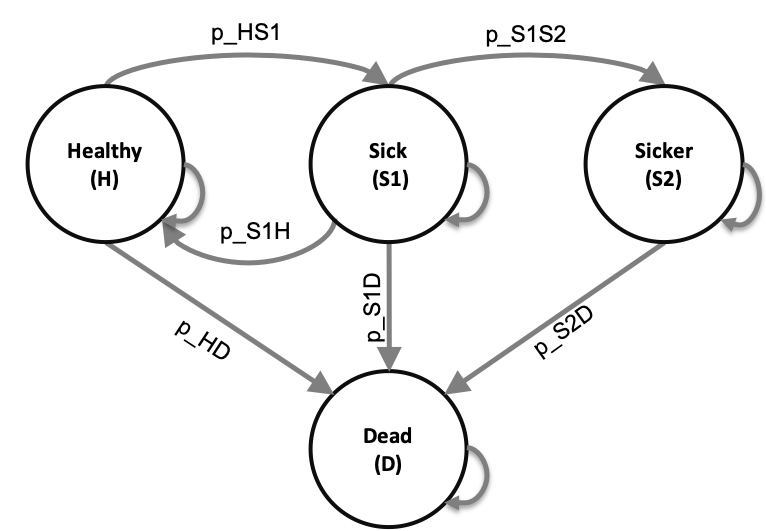
\includegraphics[width=1\linewidth]{C:/Users/Alan Yang/Desktop/GitHub local/Course-Modularization/static/Course_Modularization/Microsimulation/Microsim Sick-Sicker/figures/sick_sicker_diagram} 

}

\caption{Schematic representation of the Sick-Sicker model}\label{fig:unnamed-chunk-1}
\end{figure}

\end{document}
